
\newtoggle{inTableHeader}% Track if still in header of table
\toggletrue{inTableHeader}% Set initial value
\newcommand*{\StartTableHeader}{\global\toggletrue{inTableHeader}}%
\newcommand*{\EndTableHeader}{\global\togglefalse{inTableHeader}}%

% Redefine tabular to initialize \StartTableHeader at start and end
\let\OldTabular\tabular%
\let\OldEndTabular\endtabular%
\renewenvironment{tabular}{\StartTableHeader\OldTabular}{\OldEndTabular\StartTableHeader}%

 %The min, mid and max values
\newcommand*{\MinNumberA}{0.5}%
\newcommand*{\MidNumberA}{0.75}%
\newcommand*{\MaxNumberA}{1.0}%

%Apply the gradient macro
\newcommand{\ApplyGradientA}[1]{%
    %\IfDecimal{#1}{
  \iftoggle{inTableHeader}{#1}{
    \ifdim #1 pt > \MidNumberA pt
        \pgfmathsetmacro{\PercentColor}{max(min(100.0*(#1 - \MidNumberA)/(\MaxNumberA-\MidNumberA),100.0),0.00)} %
        \colorbox{green!\PercentColor!yellow}{#1}
    \else
        \pgfmathsetmacro{\PercentColor}{max(min(100.0*(\MidNumberA - #1)/(\MidNumberA-\MinNumberA),100.0),0.00)} %
        \colorbox{red!\PercentColor!yellow}{#1}
    \fi
  }
  %}{#1}
  }

   %The min, mid and max values
\newcommand*{\MinNumbera}{0.5}%
\newcommand*{\MidNumbera}{0.75}%
\newcommand*{\MaxNumbera}{1.0}%

%Apply the gradient macro
\newcommand{\ApplyGradienta}[1]{%
    %\IfDecimal{#1}{
  \iftoggle{inTableHeader}{#1}{
    \ifdim #1 pt > \MidNumbera pt
        \pgfmathsetmacro{\PercentColor}{max(min(100.0*(#1 - \MidNumbera)/(\MaxNumbera-\MidNumbera),100.0),0.00)} %
        \colorbox{red!\PercentColor!yellow}{#1}
    \else
        \pgfmathsetmacro{\PercentColor}{max(min(100.0*(\MidNumbera - #1)/(\MidNumbera-\MinNumbera),100.0),0.00)} %
        \colorbox{green!\PercentColor!yellow}{#1}
    \fi
  }
  %}{#1}
  }

 %The min, mid and max values
\newcommand*{\MinNumberB}{0.0}%
\newcommand*{\MidNumberB}{0.05}%
\newcommand*{\MaxNumberB}{0.1}%
  
%Apply the gradient macro
\newcommand{\ApplyGradientB}[1]{%
    %\IfDecimal{#1}{
  \iftoggle{inTableHeader}{#1}{
    \ifdim #1 pt > \MidNumberB pt
        \pgfmathsetmacro{\PercentColor}{max(min(100.0*(#1 - \MidNumberB)/(\MaxNumberB-\MidNumberB),100.0),0.00)} %
        \colorbox{red!\PercentColor!yellow}{#1}
    \else
        \pgfmathsetmacro{\PercentColor}{max(min(100.0*(\MidNumberB - #1)/(\MidNumberB-\MinNumberB),100.0),0.00)} %
        \colorbox{green!\PercentColor!yellow}{#1}
    \fi
  }
  %}{#1}
  }

%The min, mid and max values
\newcommand*{\MinNumberC}{0.5}%
\newcommand*{\MidNumberC}{0.75}%
\newcommand*{\MaxNumberC}{1.0}%
  
%Apply the gradient macro
\newcommand{\ApplyGradientC}[1]{%
    %\IfDecimal{#1}{
  \iftoggle{inTableHeader}{#1}{
    \ifdim #1 pt > \MidNumberC pt
        \pgfmathsetmacro{\PercentColor}{max(min(100.0*(#1 - \MidNumberC)/(\MaxNumberC-\MidNumberC),100.0),0.00)} %
        \colorbox{red!\PercentColor!yellow}{#1}
    \else
        \pgfmathsetmacro{\PercentColor}{max(min(100.0*(\MidNumberC - #1)/(\MidNumberC-\MinNumberC),100.0),0.00)} %
        \colorbox{green!\PercentColor!yellow}{#1}
    \fi
  }
  %}{#1}
  }

  
 %The min, mid and max values
\newcommand*{\MinNumberD}{0.5}%
\newcommand*{\MidNumberD}{0.75}%
\newcommand*{\MaxNumberD}{1.0}%

%Apply the gradient macro
\newcommand{\ApplyGradientD}[1]{%
    %\IfDecimal{#1}{
  \iftoggle{inTableHeader}{#1}{
    \ifdim #1 pt > \MidNumberD pt
        \pgfmathsetmacro{\PercentColor}{max(min(100.0*(#1 - \MidNumberD)/(\MaxNumberD-\MidNumberD),100.0),0.00)} %
        \colorbox{red!\PercentColor!yellow}{#1}
    \else
        \pgfmathsetmacro{\PercentColor}{max(min(100.0*(\MidNumberD - #1)/(\MidNumberD-\MinNumberD),100.0),0.00)} %
        \colorbox{green!\PercentColor!yellow}{#1}
    \fi
  }
  %}{#1}
  }
  
\newcolumntype{A}{>{\collectcell\ApplyGradientA}c<{\endcollectcell}}
\newcolumntype{a}{>{\collectcell\ApplyGradienta}c<{\endcollectcell}}
\newcolumntype{B}{>{\collectcell\ApplyGradientB}c<{\endcollectcell}}
\newcolumntype{C}{>{\collectcell\ApplyGradientC}c<{\endcollectcell}}
\newcolumntype{D}{>{\collectcell\ApplyGradientD}c<{\endcollectcell}}

\renewcommand{\arraystretch}{1}
\setlength{\fboxsep}{2mm} % box size
\setlength{\tabcolsep}{-4pt}

\chapter{Results}
\label{chap4}

In this chapter, we present the results achieved in triangulation of
ADE singularities, surfaces with ADE singularities and surfaces with 
sungular curves arised from CSG operations on the regular surfaces.
We measure some of the quality criteria proposed in \cite{korecova2021triangulation}
and compare our meshes in terms of quality with the meshes produced by a software 
for visualization of the implicit surfaces with ADE singularities implemented
based on the article by Richard Morris \cite{morris2003client}.
We compare the computational speed of the algorithm after the reimplementation
with the algorithm for the regular parts of the implicit surfaces 
implemented in \cite{korecova2021triangulation}.

\section{Quality criteria}
\label{sub4.1}

The following quality criteria \cite{korecova2021triangulation} are evaluated 
for the resulting mesh with uniform edge size:

\begin{enumerate}
    \item \textit{The mean ratio of the length of the sides of the triangle}
    
    The mean ratio of the length of the longest side of the triangle
    and the shortest side of the triangle shows the unoiforminy of the 
    triangles. 
    For equilateral triangle, the ratio equals exactly one. The ratio is
    greater than one for isosceles and scalene triangles. 
    The further the triangle is from equilateral triangle, the greater is the ratio.
    The number close to one indicates triangles close to the equilateral triangles,
    whereas the number greater than one indicates more non-uniform triangles in the mesh.

    \item \textit{Discrete approximation of the Hausdorff distance}
    
    To define the discrete approximation of the Hausdorff distance of the mesh and
    the implicit surface, one needs to introduce the notion of the distance of two sets
    of points.
\begin{definition} The distance $\delta$ of the point $a\in \R^3$ and the set
    $M \subset \R^3$ is defined as 
    \begin{equation}
        \delta(a, M) = \inf_{b \in M} \, d(a, b),
    \end{equation}
    where $d(a, b)$ is the Euclidean distance of two points in $\R^3$. 
\end{definition}
\begin{definition} The Hausdorff distance of two sets $N \subset \R^3$ and
    $M \subset \R^3$ is defined as
    \begin{equation}
        h(M, N) = \max \big \{\sup_{a \in M} \, \delta(a, N), \sup_{b \in N} \, \delta(M, b) \big \}.
    \end{equation}
\end{definition}
    The Hausdorff distance is numerically aproximated by taking the maximum distance
    of the gravity center of a triangle of the mesh and perpendicular projection of
    the gravity center to the triangulated surface.
    This approximation is based on the assumption, that the point on the surface
    closest to the gravity center of the triangle is the perpendicular projection of
    that point to the surface.

    The Hausdorff distance measures the accuracy of the triangulation by picking the 
    triangle, which approximates the surface the worst.

    \item \textit{The mean distance of the gravity center and its perpendicular projection}
    
    Measuring the mean distance of the gravity center and its perpendicular 
    projection shows the accuracy of the approximation globally, by taking into
    accout all triangles of the mesh rather than picking out the worst approximating 
    triangle.

    \item \textit{The mean distance of the neighbour vertices from the vertex and the 
    standard deviation of the distance from the mean}

    The standard deviation of the values from the mean value says about the 
    distibution of the values around the mean value. Small standard deviation indicates,
    that the values are close to the mean. On the contrary, bigger standard deviation
    indicates, that the values are further distributed from the mean value.

    \begin{definition}
        Given $N$ values -- $x_1, ..., x_N$, let us denote the arithmetical mean 
        of the values as $\overline{x}$. The standard deviation $\sigma$ can be calculated
        as
        \begin{equation}
            \sigma = \sqrt{\frac{1}{N} \sum\limits_{i=1}^{N}(x_i - \overline{x})^2}. 
        \end{equation}
    \end{definition}

    For the whole mesh, we are calculating the mean standard deviation from the 
    standard deviation of all points and its neighbour points in the mesh.
\end{enumerate}

\section{Comparison with SingSurf}
\label{sub4.2}

SingSurf \cite{singsurf} is a software used for visualization of two dimensional
and three dimensional models. It can work with parametric and implicit surfaces, 
while allowing to model also some of the surface singularities, including
ADE singularities. The software was implemented based on an article by 
Richard Morris \cite{morris2003client}.

\subsection{SingSurf algorithm}
\subsection{Evaluated quality criteria of the SingSurf meshes}
We compared in quality on fifteen different models. The models were chosen
to capture all categories of ADE singularities. Each pair of models was 
created to have the same axis aligned bounding box and approximately the
same number of faces. In the measurement, the invalid faces 
(the points are lying on a line) produced by SingSurf are not taken into 
account.

\subsubsection*{$A_{n--}$ singularities}
We created meshes of $A_{1--}, A_{2--}, A_{3--}$ and $A_{4--}$ singualrities.
The resulting meshes from our algorithm can be seen on the 
Figure \ref{img:46}. The resulting meshes generated by SingSurf 
can be seen on the Figure \ref{img:47}. By the look, one can tell,
that the meshes produced by us have more equilateral triangles.
On the other hand, the meshes produced by SingSurf approximate 
the surface better around the singular points.

\begin{figure}
    \centerline{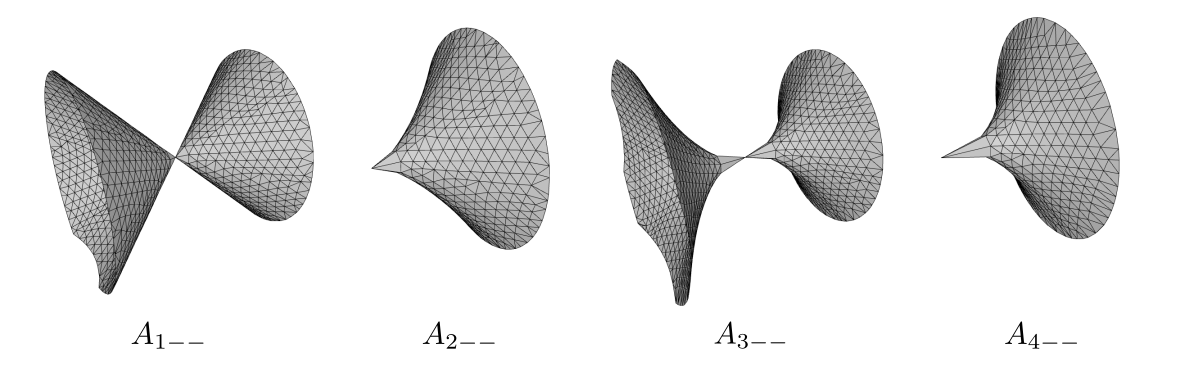
\includegraphics[scale=0.5]{images/img46}}
    \caption[Resulting triangulation of $A_{n--}$ singualrities]
    {Resulting triangulation of $A_{n--}$ singualrities.}
    %id obrazku, pomocou ktoreho sa budeme na obrazok odvolavat
    \label{img:46}
\end{figure}

\begin{figure}
    \centerline{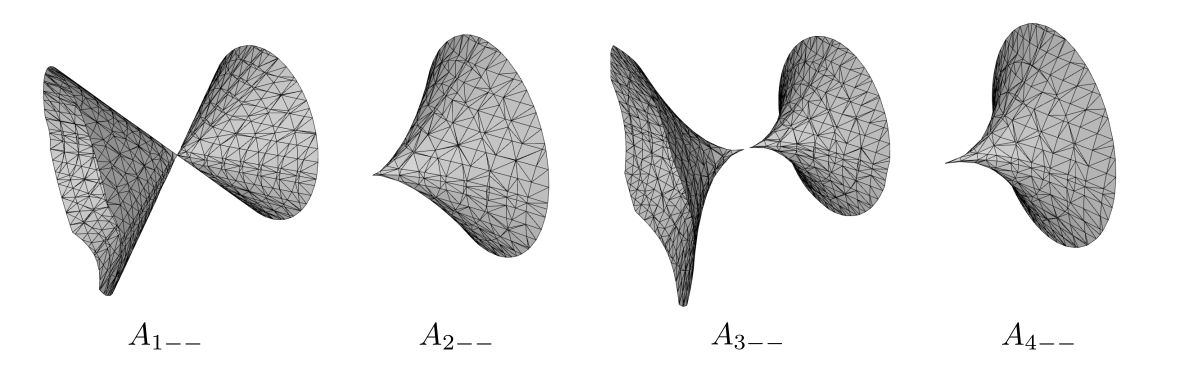
\includegraphics[scale=0.5]{images/img47}}
    \caption[Resulting triangulation of $A_{n--}$ singualrities by SingSurf]
    {Resulting triangulation of $A_{n--}$ singualrities by SingSurf \cite{singsurf}.}
    %id obrazku, pomocou ktoreho sa budeme na obrazok odvolavat
    \label{img:47}
\end{figure}

The comparison on the quality criteria measured on these meshes 
is in the table \ref{tab:An--}. The better values are visualized
by the green color and the worse values are visualized by the red 
color.

\renewcommand*{\MinNumberA}{0.0}%
\renewcommand*{\MaxNumberA}{1.0}%
\pgfmathsetmacro{\MidNumberA}{(\MinNumberA+\MaxNumberA)/2}%
\renewcommand*{\MinNumberB}{0.0}%
\renewcommand*{\MaxNumberB}{0.021}%
\pgfmathsetmacro{\MidNumberB}{(\MinNumberB+\MaxNumberB)/2}%
\renewcommand*{\MinNumberC}{0.0}%
\renewcommand*{\MaxNumberC}{0.01}%
\pgfmathsetmacro{\MidNumberC}{(\MinNumberC+\MaxNumberC)/2}%
\renewcommand*{\MinNumberD}{0.010}%
\renewcommand*{\MaxNumberD}{0.052}%
\pgfmathsetmacro{\MidNumberD}{(\MinNumberD+\MaxNumberD)/2}%


\begin{table}[ht]
    \caption[caption TODO]{caption TODO}
        \begin{center}
        \label{tab:An--}
            \begin{tabular}{|c|c|A B C D|} 
                \hline
                \hline
                \multicolumn{6}{|c|}{$A_{n--}$} \\
                \hline
                \hline
                \hspace{3mm} type \hspace{3mm} & \hspace{20mm} \hspace{20mm} & $k_1$ & $k_2$ & $k_3$ & $k_4$ \EndTableHeader\\
                \hline
                \hline
                \multirow{2}{*}{$A_{1--}$} & SingSurf & 0.113 & 0.015 & 0.001 & 0.052\\
                \cline{2-6} 
                                            & Our algorithm & 0.840 & 0.007 & 0.001 & 0.010\\
                \hline
                \hline 
                \multirow{2}{*}{$A_{2--}$} & SingSurf & 0.077 & 0.008 & 0.001 & 0.051\\
                \cline{2-6}
                                            & Our algorithm & 0.840 & 0.007 & 0.001 & 0.010\\
                \hline
                \hline
                \multirow{2}{*}{$A_{3--}$} & SingSurf & 0.049 & 0.012 & 0.001 & 0.048\\
                \cline{2-6}
                                            & Our algorithm & 0.833 & 0.013 & 0.001 & 0.011\\
                \hline
                \hline
                \multirow{2}{*}{$A_{4--}$} & SingSurf & 0.325 & 0.020 & 0.001 & 0.045\\
                \cline{2-6}
                                            & Our algorithm & 0.810 & 0.021 & 0.001 & 0.014\\
                \hline
                \hline
            \end{tabular}
        \end{center}
    \end{table}


\renewcommand*{\MinNumberA}{0.0}%
\renewcommand*{\MaxNumberA}{1.0}%
\pgfmathsetmacro{\MidNumberA}{(\MinNumberA+\MaxNumberA)/2}%
\renewcommand*{\MinNumberB}{0.008}%
\renewcommand*{\MaxNumberB}{0.061}%
\pgfmathsetmacro{\MidNumberB}{(\MinNumberB+\MaxNumberB)/2}%
\renewcommand*{\MinNumberC}{0.00}%
\renewcommand*{\MaxNumberC}{0.01}%
\pgfmathsetmacro{\MidNumberC}{(\MinNumberC+\MaxNumberC)/2}% 
\renewcommand*{\MinNumberD}{0.011}%
\renewcommand*{\MaxNumberD}{0.118}%
\pgfmathsetmacro{\MidNumberD}{(\MinNumberD+\MaxNumberD)/2}%


\begin{table}[ht]
    \caption[caption TODO]{caption TODO}
        \begin{center}
        \label{tab:An--}
            \begin{tabular}{|c|c|A B C D|} 
                \hline
                \hline
                \multicolumn{6}{|c|}{$A_{n--}$} \\
                \hline
                \hline
                \hspace{3mm} type \hspace{3mm} & \hspace{20mm} \hspace{20mm} & $k_1$ & $k_2$ & $k_3$ & $k_4$ \EndTableHeader\\
                \hline
                \hline
                \multirow{2}{*}{$A_{2+-}$} & SingSurf       & 0.189 & 0.017 & 0.002 & 0.052\\
                \cline{2-6}
                                            & Our algorithm & 0.835 & 0.008 & 0.002 & 0.011\\
                \hline
                \hline
                \multirow{2}{*}{$A_{3+-}$} & SingSurf       & 0.001 & 0.042 & 0.005 & 0.073\\
                \cline{2-6}
                                            & Our algorithm & 0.824 & 0.013 & 0.002 & 0.015\\
                \hline
                \hline
                \multirow{2}{*}{$A_{4+-}$} & SingSurf       & 0.001 & 0.061 & 0.006 & 0.118\\
                \cline{2-6}
                                            & Our algorithm & 0.820 & 0.033 & 0.006 & 0.031\\
                \hline
                \hline 
            \end{tabular}
        \end{center} 
    \end{table}
    
\renewcommand*{\MinNumberA}{0.0}%
\renewcommand*{\MaxNumberA}{1.0}%
\pgfmathsetmacro{\MidNumberA}{(\MinNumberA+\MaxNumberA)/2}%
\renewcommand*{\MinNumberB}{0.017}%
\renewcommand*{\MaxNumberB}{0.032}%
\pgfmathsetmacro{\MidNumberB}{(\MinNumberB+\MaxNumberB)/2}%
\renewcommand*{\MinNumberC}{0.0}%
\renewcommand*{\MaxNumberC}{0.01}%
\pgfmathsetmacro{\MidNumberC}{(\MinNumberC+\MaxNumberC)/2}% 
\renewcommand*{\MinNumberD}{0.009}%
\renewcommand*{\MaxNumberD}{0.078}%
\pgfmathsetmacro{\MidNumberD}{(\MinNumberD+\MaxNumberD)/2}%


\begin{table}[ht]
    \caption[caption TODO]{caption TODO}
        \begin{center}
        \label{tab:An--}
        \begin{tabular}{|c|c|A B C D|} 
            \hline
            \hline
            \multicolumn{6}{|c|}{$A_{n--}$} \\
            \hline
            \hline
            \hspace{3mm} type \hspace{3mm} & \hspace{20mm} \hspace{20mm} & $k_1$ & $k_2$ & $k_3$ & $k_4$ \EndTableHeader\\
            \hline
            \hline
            \multirow{2}{*}{$D_{4--}$} & SingSurf       & 0.091 & 0.017 & 0.002 & 0.052\\
            \cline{2-6}
                                        & Our algorithm & 0.794 & 0.024 & 0.002 & 0.009\\
            \hline
            \hline
            \multirow{2}{*}{$D_{4+-}$} & SingSurf       & 0.094 & 0.028 & 0.003 & 0.078\\
            \cline{2-6}
                                        & Our algorithm & 0.855 & 0.022 & 0.002 & 0.019\\
            \hline
            \hline
            \multirow{2}{*}{$D_{5--}$} & SingSurf       & 0.001 & 0.032 & 0.006 & 0.076\\
            \cline{2-6}
                                        & Our algorithm & 0.789 & 0.029 & 0.005 & 0.022\\
            \hline
            \hline 
            \multirow{2}{*}{$D_{5+-}$} & SingSurf       & 0.132 & 0.029 & 0.003 & 0.076\\
            \cline{2-6}
                                        & Our algorithm & 0.831 & 0.021 & 0.002 & 0.020\\
            \hline
            \hline 
        \end{tabular}
    \end{center} 
\end{table}

    
\renewcommand*{\MinNumberA}{0.0}%
\renewcommand*{\MaxNumberA}{1.0}%
\pgfmathsetmacro{\MidNumberA}{(\MinNumberA+\MaxNumberA)/2}%
\renewcommand*{\MinNumberB}{0.017}%
\renewcommand*{\MaxNumberB}{0.059}%
\pgfmathsetmacro{\MidNumberB}{(\MinNumberB+\MaxNumberB)/2}%
\renewcommand*{\MinNumberC}{0.0}%
\renewcommand*{\MaxNumberC}{0.01}%
\pgfmathsetmacro{\MidNumberC}{(\MinNumberC+\MaxNumberC)/2}% 
\renewcommand*{\MinNumberD}{0.014}%
\renewcommand*{\MaxNumberD}{0.110}%
\pgfmathsetmacro{\MidNumberD}{(\MinNumberD+\MaxNumberD)/2}%


\begin{table}[ht]
    \caption[caption TODO]{caption TODO}
        \begin{center}
        \label{tab:En}
        \begin{tabular}{|c|c|A B C D|} 
            \hline
            \hline
            \multicolumn{6}{|c|}{$E_{n}$ singularities} \\
            \hline
            \hline
            \hspace{3mm} type \hspace{3mm} & \hspace{20mm} \hspace{20mm} & $k_1$ & $k_2$ & $k_3$ & $k_4$ \EndTableHeader\\
            \hline
            \hline
            \multirow{2}{*}{$E_{6++}$} & SingSurf       & 0.006 & 0.043 & 0.003 & 0.069\\
            \cline{2-6}
                                        & Our algorithm & 0.858 & 0.017 & 0.002 & 0.014\\
            \hline
            \hline
            \multirow{2}{*}{$E_{6+-}$} & SingSurf       & 0.011 & 0.040 & 0.003 & 0.077\\
            \cline{2-6}
                                        & Our algorithm & 0.403 & 0.021 & 0.002 & 0.019\\
            \hline
            \hline
            \multirow{2}{*}{$E_{7++}$} & SingSurf       & 0.198 & 0.024 & 0.004 & 0.110\\
            \cline{2-6}
                                        & Our algorithm & 0.803 & 0.059 & 0.004 & 0.030\\
            \hline
            \hline 
            \multirow{2}{*}{$E_{8++}$} & SingSurf       & 0.260 & 0.045 & 0.004 & 0.100\\
            \cline{2-6}
                                        & Our algorithm & 0.828 & 0.044 & 0.004 & 0.029\\
            \hline 
            \hline 
        \end{tabular}
    \end{center} 
\end{table}
\section{Computational speed comparison of the reimplemented solution}
\label{sub4.3}